\documentclass[10pt,onecolumn,letterpaper]{article}

\usepackage{cvpr}
\usepackage{times}
\usepackage{epsfig}
\usepackage{graphicx}
\usepackage{grffile}
\usepackage{amsmath}
\usepackage{amssymb}
\usepackage{amsmath}
\usepackage{amsfonts}
\usepackage{subfigure}
\usepackage{nonfloat}
\usepackage{url}
\usepackage[colorlinks=true, linkcolor=green, pagebackref]{hyperref}
\usepackage{textcomp} % for textonehalf

\usepackage{wrapfig}
\graphicspath{{../report/imgs/}{./imgs/}{./imgs/bigbird/new_turntables/}{./imgs/bigbird/rgb_ims/}} %renders_turn_table_new/}}

\usepackage{xspace}
\renewcommand*{\eg}{e.g.\@\xspace}
\renewcommand*{\ie}{i.e.\@\xspace}
\newcommand*{\ea}{et al.\@\xspace}
\renewcommand*{\vs}{vs.\@\xspace}

\def\cvprPaperID{1437} % *** Enter the CVPR Paper ID here
\def\httilde{\mbox{\tt\raisebox{-.5ex}{\symbol{126}}}}

\definecolor{red}{rgb}{0.95,0.4,0.4}
\definecolor{blue}{rgb}{0.4,0.4,0.95}

\newcommand{\todo}[1]{\textcolor{red}{TODO: #1}}
\newcommand{\note}[1]{\textcolor{blue}{NOTE: #1}}

\title{Structured Prediction of Unobserved Voxels From a Single Depth Image: Supplementary Material}

\begin{document}

\maketitle

Here we present additional results from our algorithm, from the two datasets we presented results for in the main paper.
We additionally present results from running the same algorithm on a third dataset.

%%%%%%%%%%%%%%%%%%%%%%%%%%%%%%%%%%%%%%%%%%%%%%%%%%%%%%%%
\section{`Bigbird' turntable dataset results}


\newcommand{\turnheight}{0.12\columnwidth}

\begin{tabular}{cccccc}
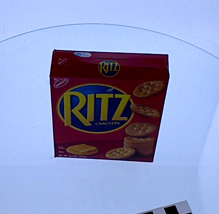
\includegraphics[height=\turnheight, clip=true, trim=20 30 30 5]{ritz_crackers.png} &
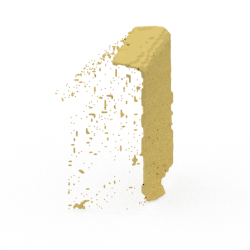
\includegraphics[height=\turnheight, clip=true, trim=60 30 30 5]{ritz_crackers_NP3_0_visible_pixels_view_180.png} &
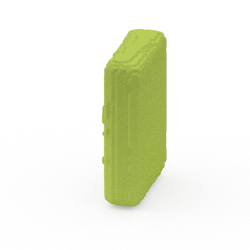
\includegraphics[height=\turnheight, clip=true, trim=60 30 30 5]{ritz_crackers_NP3_0_gt_view_180.png} &
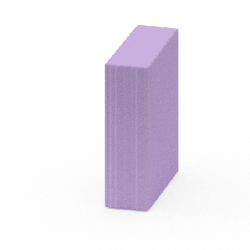
\includegraphics[height=\turnheight, clip=true, trim=60 30 30 5]{ritz_crackers_NP3_0_bb_view_180.png} &
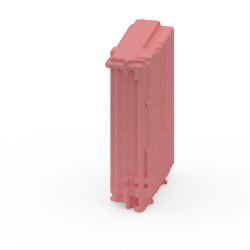
\includegraphics[height=\turnheight, clip=true, trim=60 30 30 5]{ritz_crackers_NP3_0_zheng_view_180.png} &
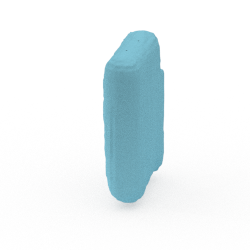
\includegraphics[height=\turnheight, clip=true, trim=60 30 30 5]{ritz_crackers_NP3_0_oma_view_180} \\
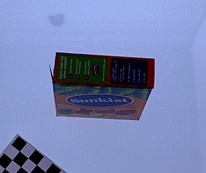
\includegraphics[height=\turnheight, clip=true, trim=20 30 30 5]{sunkist_fruit_snacks_mixed_fruit.png} &
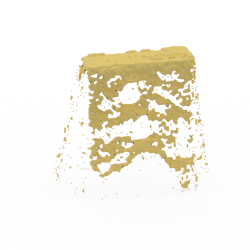
\includegraphics[height=\turnheight, clip=true, trim=60 30 30 5]{sunkist_fruit_snacks_mixed_fruit_NP4_0_visible_pixels_view_90.png} &
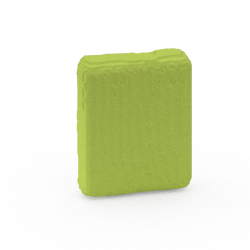
\includegraphics[height=\turnheight, clip=true, trim=60 30 30 5]{sunkist_fruit_snacks_mixed_fruit_NP4_0_gt_view_90.png} &
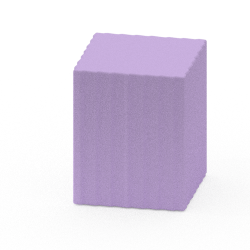
\includegraphics[height=\turnheight, clip=true, trim=60 30 30 5]{sunkist_fruit_snacks_mixed_fruit_NP4_0_bb_view_90.png} &
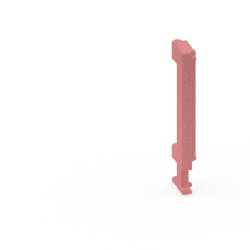
\includegraphics[height=\turnheight, clip=true, trim=60 30 30 5]{sunkist_fruit_snacks_mixed_fruit_NP4_0_zheng_view_90.png} &
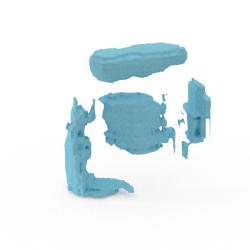
\includegraphics[height=\turnheight, clip=true, trim=60 30 30 5]{sunkist_fruit_snacks_mixed_fruit_NP4_0_oma_view_90} \\
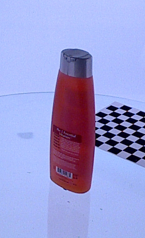
\includegraphics[height=\turnheight, clip=true, trim=20 30 30 5]{vo5_extra_body_volumizing_shampoo.png} &
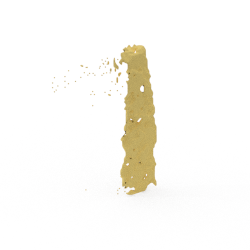
\includegraphics[height=\turnheight, clip=true, trim=60 30 30 5]{vo5_extra_body_volumizing_shampoo_NP2_216_visible_pixels_view_0.png} &
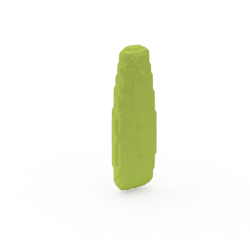
\includegraphics[height=\turnheight, clip=true, trim=60 30 30 5]{vo5_extra_body_volumizing_shampoo_NP2_216_gt_view_0.png} &
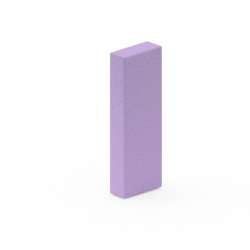
\includegraphics[height=\turnheight, clip=true, trim=60 30 30 5]{vo5_extra_body_volumizing_shampoo_NP2_216_bb_view_0.png} &
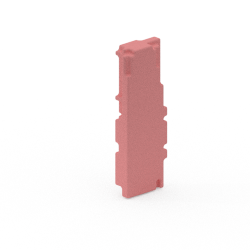
\includegraphics[height=\turnheight, clip=true, trim=60 30 30 5]{vo5_extra_body_volumizing_shampoo_NP2_216_zheng_view_0.png} &
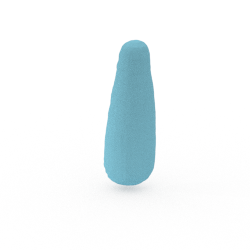
\includegraphics[height=\turnheight, clip=true, trim=60 30 30 5]{vo5_extra_body_volumizing_shampoo_NP2_216_oma_view_0} \\
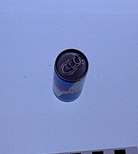
\includegraphics[height=\turnheight, clip=true, trim=20 30 30 5]{red_bull.png} &
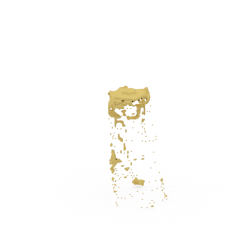
\includegraphics[height=\turnheight, clip=true, trim=60 30 30 5]{red_bull_NP4_0_visible_pixels_view_270.png} &
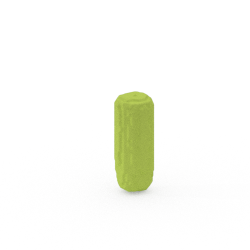
\includegraphics[height=\turnheight, clip=true, trim=60 30 30 5]{red_bull_NP4_0_gt_view_270.png} &
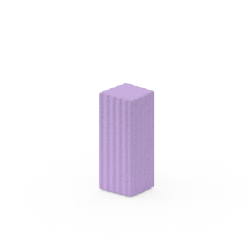
\includegraphics[height=\turnheight, clip=true, trim=60 30 30 5]{red_bull_NP4_0_bb_view_270.png} &
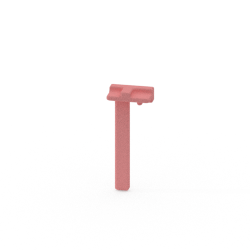
\includegraphics[height=\turnheight, clip=true, trim=60 30 30 5]{red_bull_NP4_0_zheng_view_270.png} &
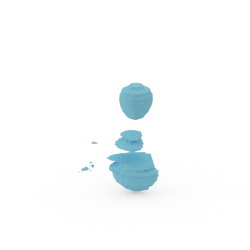
\includegraphics[height=\turnheight, clip=true, trim=60 30 30 5]{red_bull_NP4_0_oma_view_270} \\
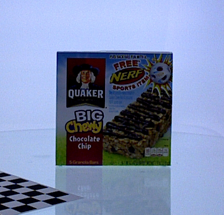
\includegraphics[height=\turnheight, clip=true, trim=20 30 30 5]{quaker_big_chewy_chocolate_chip.png} &
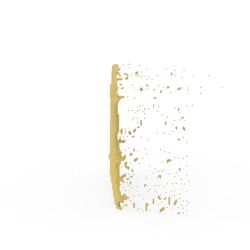
\includegraphics[height=\turnheight, clip=true, trim=60 30 30 5]{quaker_big_chewy_chocolate_chip_NP1_0_visible_pixels_view_0.png} &
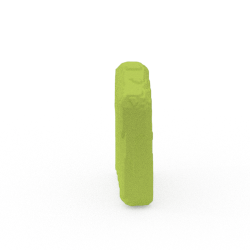
\includegraphics[height=\turnheight, clip=true, trim=60 30 30 5]{quaker_big_chewy_chocolate_chip_NP1_0_gt_view_0.png} &
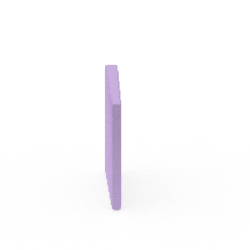
\includegraphics[height=\turnheight, clip=true, trim=60 30 30 5]{quaker_big_chewy_chocolate_chip_NP1_0_bb_view_0.png} &
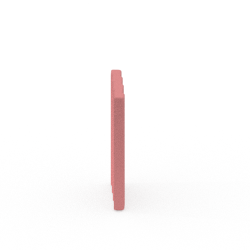
\includegraphics[height=\turnheight, clip=true, trim=60 30 30 5]{quaker_big_chewy_chocolate_chip_NP1_0_zheng_view_0.png} &
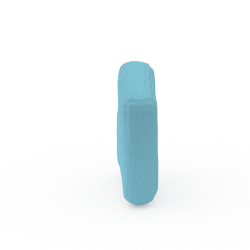
\includegraphics[height=\turnheight, clip=true, trim=60 30 30 5]{quaker_big_chewy_chocolate_chip_NP1_0_oma_view_0} \\
\includegraphics[height=\turnheight, clip=true, trim=20 30 30 5]{pringles_bbq.png} &
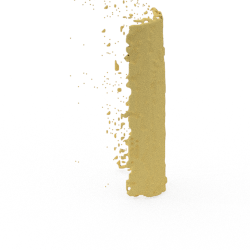
\includegraphics[height=\turnheight, clip=true, trim=60 30 30 5]{pringles_bbq_NP1_312_visible_pixels_view_180.png} &
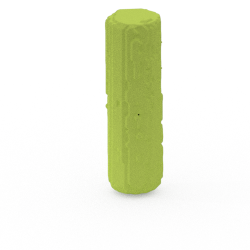
\includegraphics[height=\turnheight, clip=true, trim=60 30 30 5]{pringles_bbq_NP1_312_gt_view_180.png} &
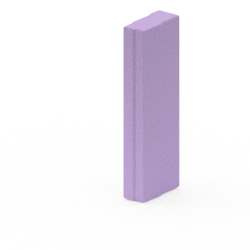
\includegraphics[height=\turnheight, clip=true, trim=60 30 30 5]{pringles_bbq_NP1_312_bb_view_180.png} &
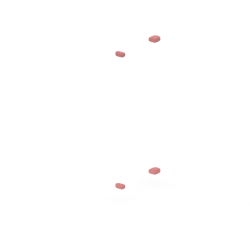
\includegraphics[height=\turnheight, clip=true, trim=60 30 30 5]{pringles_bbq_NP1_312_zheng_view_180.png} &
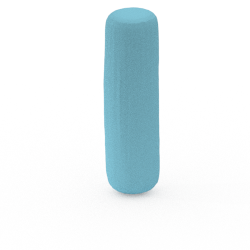
\includegraphics[height=\turnheight, clip=true, trim=60 30 30 5]{pringles_bbq_NP1_312_oma_view_180} \\
\includegraphics[height=\turnheight, clip=true, trim=20 30 30 5]{pringles_bbq.png} &
\includegraphics[height=\turnheight, clip=true, trim=60 30 30 5]{pringles_bbq_NP4_0_visible_pixels_view_0.png} &
\includegraphics[height=\turnheight, clip=true, trim=60 30 30 5]{pringles_bbq_NP4_0_gt_view_0.png} &
\includegraphics[height=\turnheight, clip=true, trim=60 30 30 5]{pringles_bbq_NP4_0_bb_view_0.png} &
\includegraphics[height=\turnheight, clip=true, trim=60 30 30 5]{pringles_bbq_NP4_0_zheng_view_0.png} &
\includegraphics[height=\turnheight, clip=true, trim=60 30 30 5]{pringles_bbq_NP4_0_oma_view_0} \\
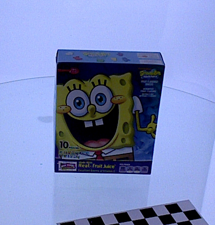
\includegraphics[height=\turnheight, clip=true, trim=20 30 30 5]{spongebob_squarepants_fruit_snaks.png} &
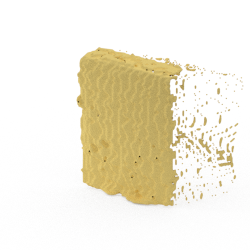
\includegraphics[height=\turnheight, clip=true, trim=60 30 30 5]{spongebob_squarepants_fruit_snaks_NP2_0_visible_pixels_view_90.png} &
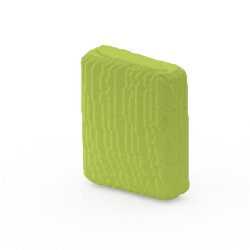
\includegraphics[height=\turnheight, clip=true, trim=60 30 30 5]{spongebob_squarepants_fruit_snaks_NP2_0_gt_view_90.png} &
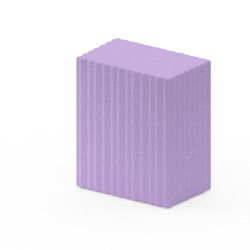
\includegraphics[height=\turnheight, clip=true, trim=60 30 30 5]{spongebob_squarepants_fruit_snaks_NP2_0_bb_view_90.png} &
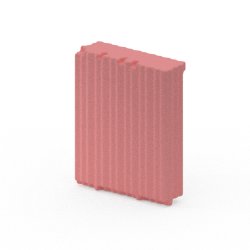
\includegraphics[height=\turnheight, clip=true, trim=60 30 30 5]{spongebob_squarepants_fruit_snaks_NP2_0_zheng_view_90.png} &
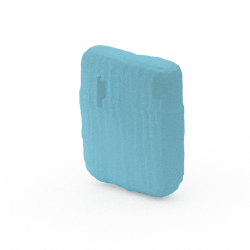
\includegraphics[height=\turnheight, clip=true, trim=60 30 30 5]{spongebob_squarepants_fruit_snaks_NP2_0_oma_view_90} \\
     Input view & Input depth pixels & Ground truth mesh & Bounding box &  Zheng \ea & Our result \\
\end{tabular}

%    \vspace{5pt}
%     \caption{Results from the Bigbird turntable dataset. 
 %    Each row shows a different object, while each column shows the result of a different algorithm.
 %     The first column shows the RGB image of the input view, while the second column shows the reprojected input depth pixels from a side view.
 %    The following columns, all shown from the same viewpoint as the input depth pixels view, demonstrate the different baselines and algorithm variants. 
 %     More views and objects can be seen in the supplementary material.
 %%    \label{fig:turntable_qual}
   %  }


% 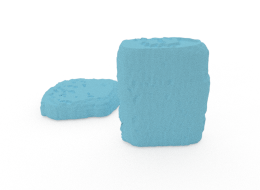
\includegraphics[width=\scenewidth]{scene/cropped/learn12_op_0} &
% 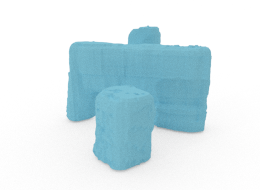
\includegraphics[width=\scenewidth]{scene/cropped/test11_op_0} &
% \includegraphics[width=\scenewidth]{scene/cropped/learn13_op_0} &
% \includegraphics[width=\scenewidth]{scene/cropped/test45_op_0} \\
% \includegraphics[width=\scenewidth]{scene/cropped/learn12_op_1} &
% \includegraphics[width=\scenewidth]{scene/cropped/test11_op_1} &
% \includegraphics[width=\scenewidth]{scene/cropped/learn13_op_1} &
% \includegraphics[width=\scenewidth]{scene/cropped/test45_op_1} \\
%\end{tabular}




\end{document}